\documentclass[compsoc]{IEEEtran}
\usepackage{graphicx}
\usepackage{amsmath}
\usepackage{authblk}
\usepackage[english]{babel}
\usepackage{blindtext}
%\usepackage[ruled,vlined,linesnumbered]{algorithm2e}
%\usepackage{algorithmic,float}
\usepackage{setspace}
\usepackage{amsfonts}
%\usepackage{hyperref}
\graphicspath{ {../images/} }
\usepackage{subfig}
\usepackage{fontspec}
\usepackage{listings}
\usepackage{amsmath}
\usepackage{mathabx}
\usepackage[bottom]{footmisc}
\newfontfamily\listingsfont[Scale=.7]{inconsolata}\usepackage[font=footnotesize,labelfont=bf]{caption}
%\captionsetup[algorithm2e]{font=footnotesize}
\usepackage[table,xcdraw]{xcolor}
\usepackage[utf8]{inputenc}
\title{Assignment: Transfer Learning on Intel Image Classification}
\author{David Bertoldi -- 735213 \\ email: d.bertoldi@campus.unimib.it}
\affil{Department of Informatics, Systems and Communication}
\affil{University of Milano-Bicocca}
\date{October 2022}


\begin{document}

\maketitle 



\section{Dataset}\label{sec:insp}
The chosen dataset is called Intel$^\circledR$ Image Classification and it was initially published on Analytics Vidhya by Intel$^\circledR$ to host an image classification challenge to promote OpenVINO™, a toolkit or optimizing and deploying AI inference \cite{site1}\cite{site2}. \par

The dataset contains images of natural scenes around the world and they belong to $6$ classes: buildings, forests, glaciers, mountains, sea and streets. The images are of size $150\times150$px and can be colored ($3$ channels, RGB) or rarely in grayscale (still with $3$ channels). Figure \ref{fig:samples} shows $16$ entries of the training dataset. \par
There is a total of ${\sim 24\,000}$ images, divided into Train (${\sim14\,000}$), Test (${\sim3\,000}$) and Prediction (${\sim7\,000}$) folders. The last one does not contain labels and it is intended for unsupervised learning and it will be ignored in this work.



\begin{figure}[ht!]
\centering                                                                        
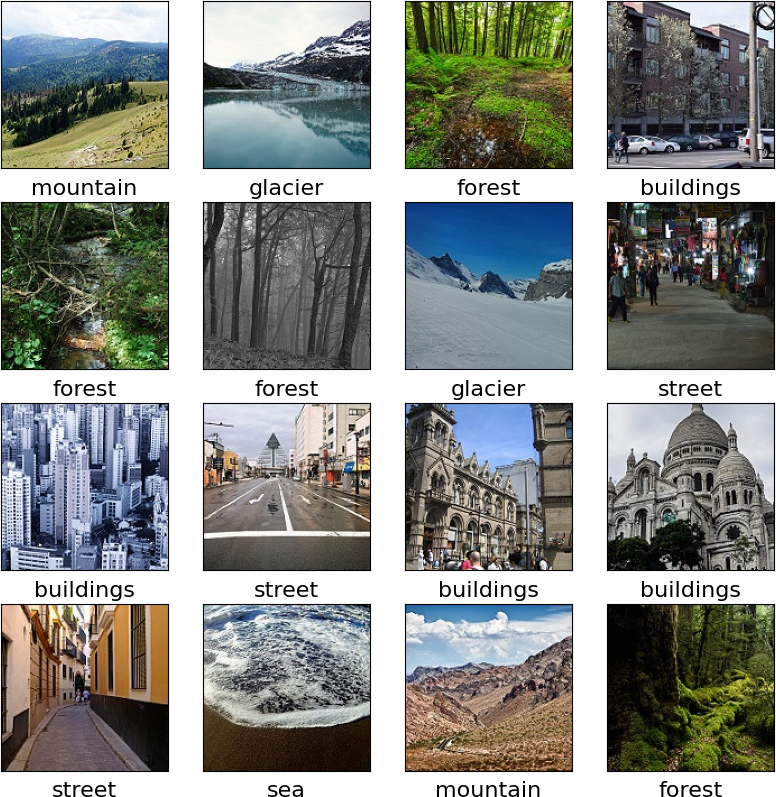
\includegraphics[width=2.5in]{../images/samples.png}
\captionsetup{justification=centering}                                                                                         
\caption{$16$ random entries of the train dataset}
\label{fig:samples}                                                                                                                               
\end{figure}

The distribution of the images across the classes follows a uniform distribution $U(\mu, \sigma)$: in the train set each class has an average $\mu = 2\,339$ images with $\sigma = 105.45$ and in the test set $\mu=500$ and $\sigma=36.92$. We didn't find any bias inside the dataset since all the classes are equally populated and so we didn't applied any kind of data augmentation on particular classes for rebalacing.


\begin{figure}[ht!]
\centering                                                                        
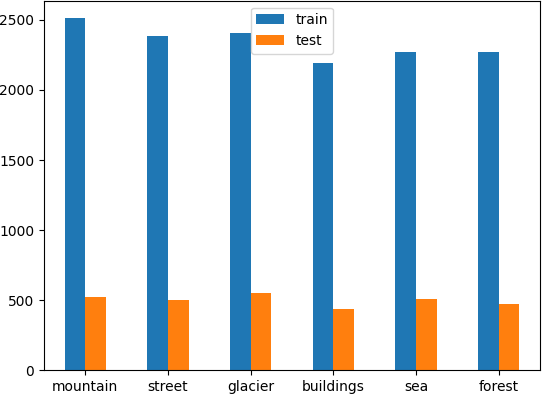
\includegraphics[width=3in]{../images/data.png}
\captionsetup{justification=centering}                                                                                         
\caption{16 entries of the train dataset}
\label{fig:data}                                                                                                                               
\end{figure}

The $6$ classes are encoded with numbers $0$ to $5$ and Table \ref{tab:encode} shows the mapping between the numerical and nominative form.



\begin{table}[ht!]
\centering
\begin{tabular}{|l|l|}
\hline
\rowcolor[HTML]{9698ED} 
{\color[HTML]{FFFFFF} \textbf{Number}} & {\color[HTML]{FFFFFF} \textbf{Class}} \\ \hline
0                                      & Mountain                              \\ \hline
1                                      & Street                                \\ \hline
2                                      & Glacier                               \\ \hline
3                                      & Building                              \\ \hline
4                                      & Sea                                   \\ \hline
5                                      & Forest                                \\ \hline
\end{tabular}
\caption{Mapping between numbers and names}
\label{tab:encode}
\end{table}



\section{The model} 
The chosen dataset presented similarieties with ImageNet: the $6$ classes of Intel$^\circledR$ Image Classification are scattered and distributed in the $1\,000$ classes of ImageNet. For this reason a pretrained model on ImageNet speeded up the learning process. The chosen model is VGG16, a $16-$layers deep CNN proposed by Karen Simonyan and Andrew Zisserman at the University of Oxford\cite{vgg16}. Figure \ref{fig:vgg16} shows an overview of its architecture.


\begin{figure}[ht!]
\centering                                                                        
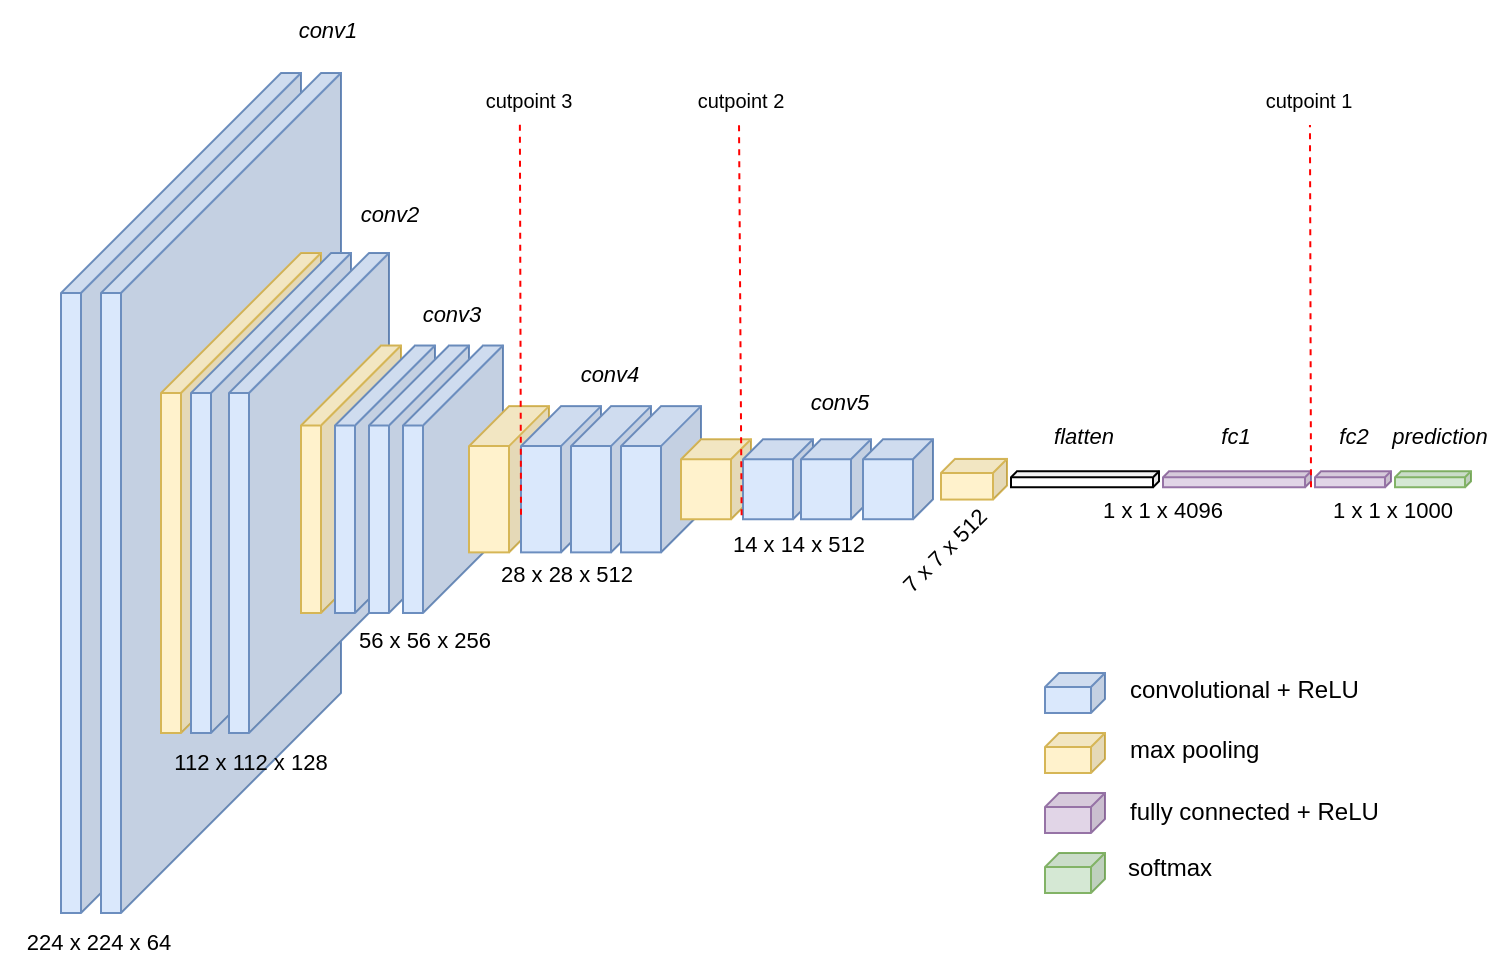
\includegraphics[width=3.5in]{../images/vgg16.png}
\captionsetup{justification=centering}                                                                                         
\caption{Architecture of VGG16 with the cuts applied in this work}
\label{fig:vgg16}                                                                                                                               
\end{figure}

In this work we proposed different cuts to the network and feeded its outputs to a "classic" machine learning model, a SVM, and benchmark the performance of the hybrid architecture. \par

The chosen cuts were after the first dense layer (\texttt{fc1}), after the fourth pooling layer (\texttt{block4\_pool}) 
and after the third pooling layer (\texttt{block3\_pool}). The different cuts led to different challenges, such as the high dimensionality of the features.


As the cuts approached the input, the number of trainable parameters decreased exponentially; however the representation of the features will have an increasingly higher dimension. The higher dimensionality affects the training performance of the SVM and a fine tuning on the management of the memory. For this reason we used less samples during the training phase as the dimensionality increased, raising the risk of underfitting. Table \ref{tab:dims} describes the numbers of the problems.


\begin{table}[]
\centering
\resizebox{\columnwidth}{!}{%
\begin{tabular}{|l|c|l|}
\hline
\rowcolor[HTML]{9698ED} 
{\color[HTML]{FFFFFF} \textbf{Cut}} & {\color[HTML]{FFFFFF} \textbf{Trainable parameters}} & {\color[HTML]{FFFFFF} \textbf{Dimension}} \\ \hline
\texttt{fc1}                                 & $117\,479\,232$  & $1\times1\times4096=\mathbf{4\,096}$                             \\ \hline
\texttt{block4\_pool}                        & $7\,635\,264$  & $14\times14\times512 = \mathbf{100\,352}$                      \\ \hline
\texttt{block3\_pool}                        & $1\,735\,488$  & $28\times28\times256= \mathbf{200\,704}$                         \\ \hline
\end{tabular}}
\caption{Number of VGG16's trainable parameters and dimensions of the extracted features at each cutting point}
\label{tab:dims}
\end{table}




\section{First cutting point: \texttt{fc1}}\label{sec:fc1}

Before attaching to the layer \texttt{fc1} the SVM, it is interesting to visualize the features through PCA (Principal Component Analysis): we decreased the number of dimensions of the extracted features from $4\,096$ to $2$ and plotted the graph in Figure \ref{fig:pca1}.

\begin{figure}[ht!]
\centering                                                                        
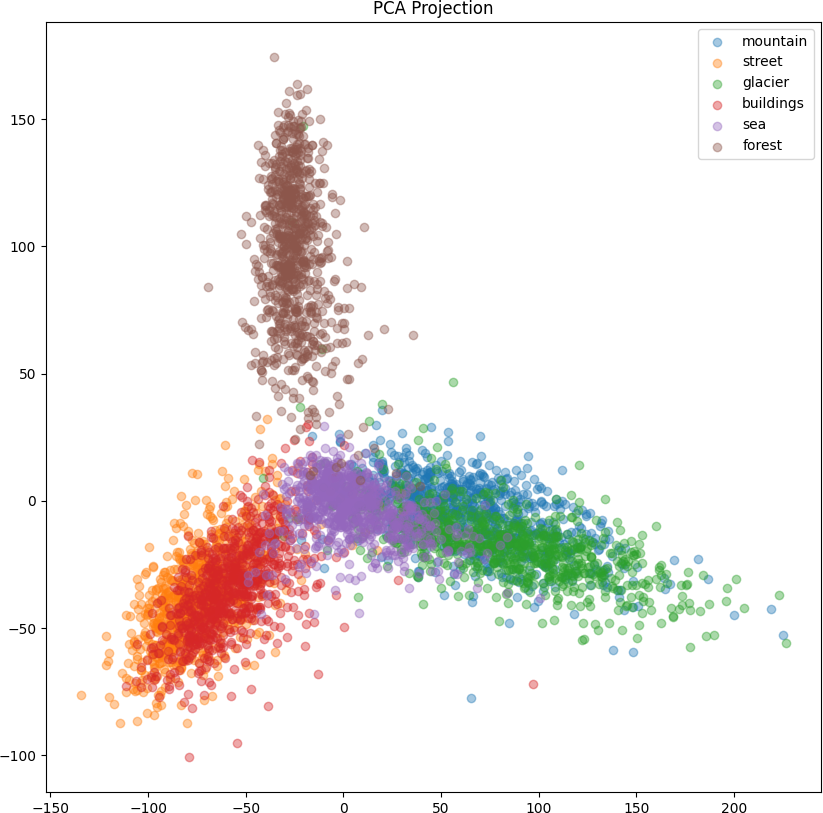
\includegraphics[width=3.5in]{../images/pca-1.png}
\captionsetup{justification=centering}                                                                                         
\caption{Architecture of VGG16 with the cuts applied in this work}
\label{fig:pca1}                                                                                                                               
\end{figure}

In the projection through PCA are identifiable some clusters: glaciers and mountains are very similar, the same goes for streets and buildings. This make sense since the picture of the mountains may contain snow or ice and picture of buildings may contain the surrounding street, and viceversa. The seas borders with the glaciers but it does not blend with them. The forests are a separate concepts and it seems to not share anything with the other classes. \par
Because the cut is very close to the VGG16's original output we expected an high accuracy in classifying the images.




\subsection{Extraction of the features and training of the SVM}
Before starting with the training of the hybrid model, we chose the SVM's hyperparameters using \texttt{GridSearchCV} from sklearn. This function does an exhaustive search of the best parameters for the SVM in order to find the best separation hyperplane. The parameters to be chosen were the cost $C \in \{5, 10, 20, 100\}$ and the kernel coefficient $\gamma \in \{scale, auto\}$. This does not assure that it gives back the best configurations on unseen data. As a matter of fact we should had the best results with cost $C=100$ and $\gamma=auto$ (Figure \ref{fig:costs}), but in this case we achieved higher performances on the test dataset with $C=100$ and $\gamma=scale$. So we used \texttt{GridSearchCV} just like a starting point for further manual experimentations.

\begin{figure}[ht!]
\centering                                                                        
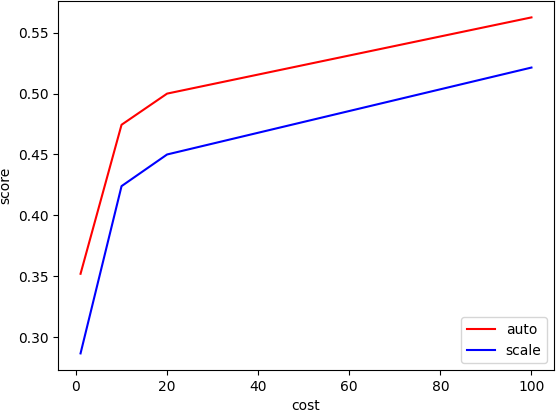
\includegraphics[width=3in]{../images/costs.png}
\captionsetup{justification=centering}                                                                                         
\caption{Model's performance on the training set with different configurations}
\label{fig:costs}                                                                                                                               
\end{figure}

An issue when using hybrid models are some incompatabilities between libraries: we started using Tensorflow's \texttt{DirectoryIterator} or \texttt{Dataset} in order to efficiently load the dataset in batches and to not saturate the memory; unfortunately sklearn does not support this kind of data structure and the only feasible solution was to diminuish the number of samples during the training and test phases. With this cutting point we used $1\,000$ images per class when training and $450$ when testing. \par
The training accuracy reached $100\%$ and Figure \ref{fig:cm1-train} shows the confusion matrix. 


\begin{figure}[ht!]
\centering                                                                        
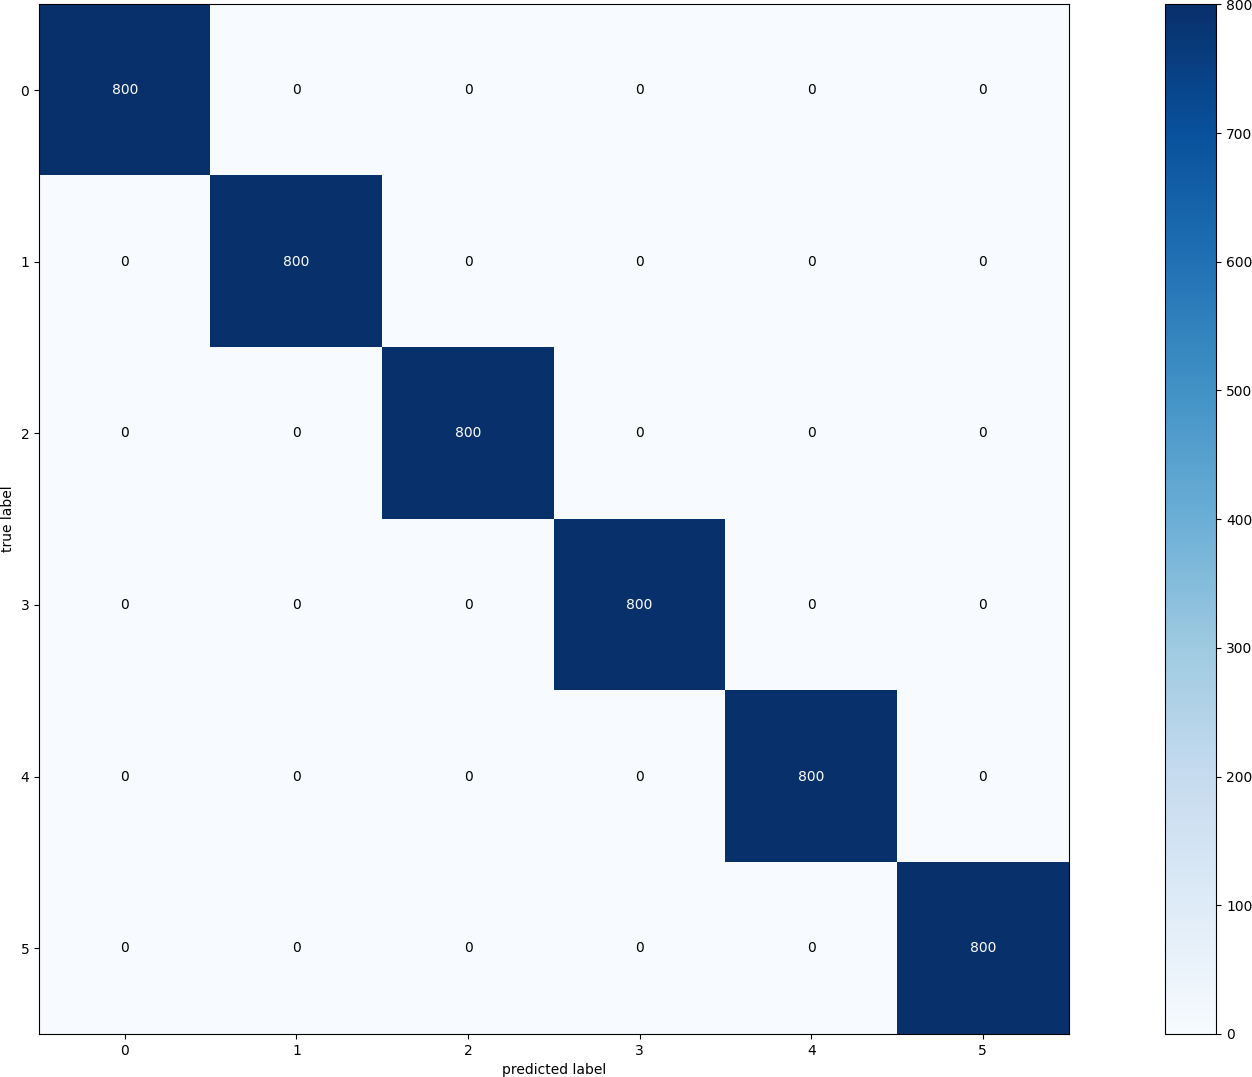
\includegraphics[width=3in]{../images/cm1-train.png}
\captionsetup{justification=centering}                                                                                         
\caption{Confusion matrix on training dataset \\ (cut at \texttt{fc1} + SVM($C=100, \gamma=scale$))}
\label{fig:cm1-train}                                                                                                                               
\end{figure}

The test accuracy reached $92\%$ and Figure \ref{fig:cm1-test} shows the confusion matrix. We can notice a little confusion between mountains and glaciers and between streets and buildings. This results are in accordance with Figure \ref{fig:pca1}.


\begin{figure}[ht!]
\centering                                                                        
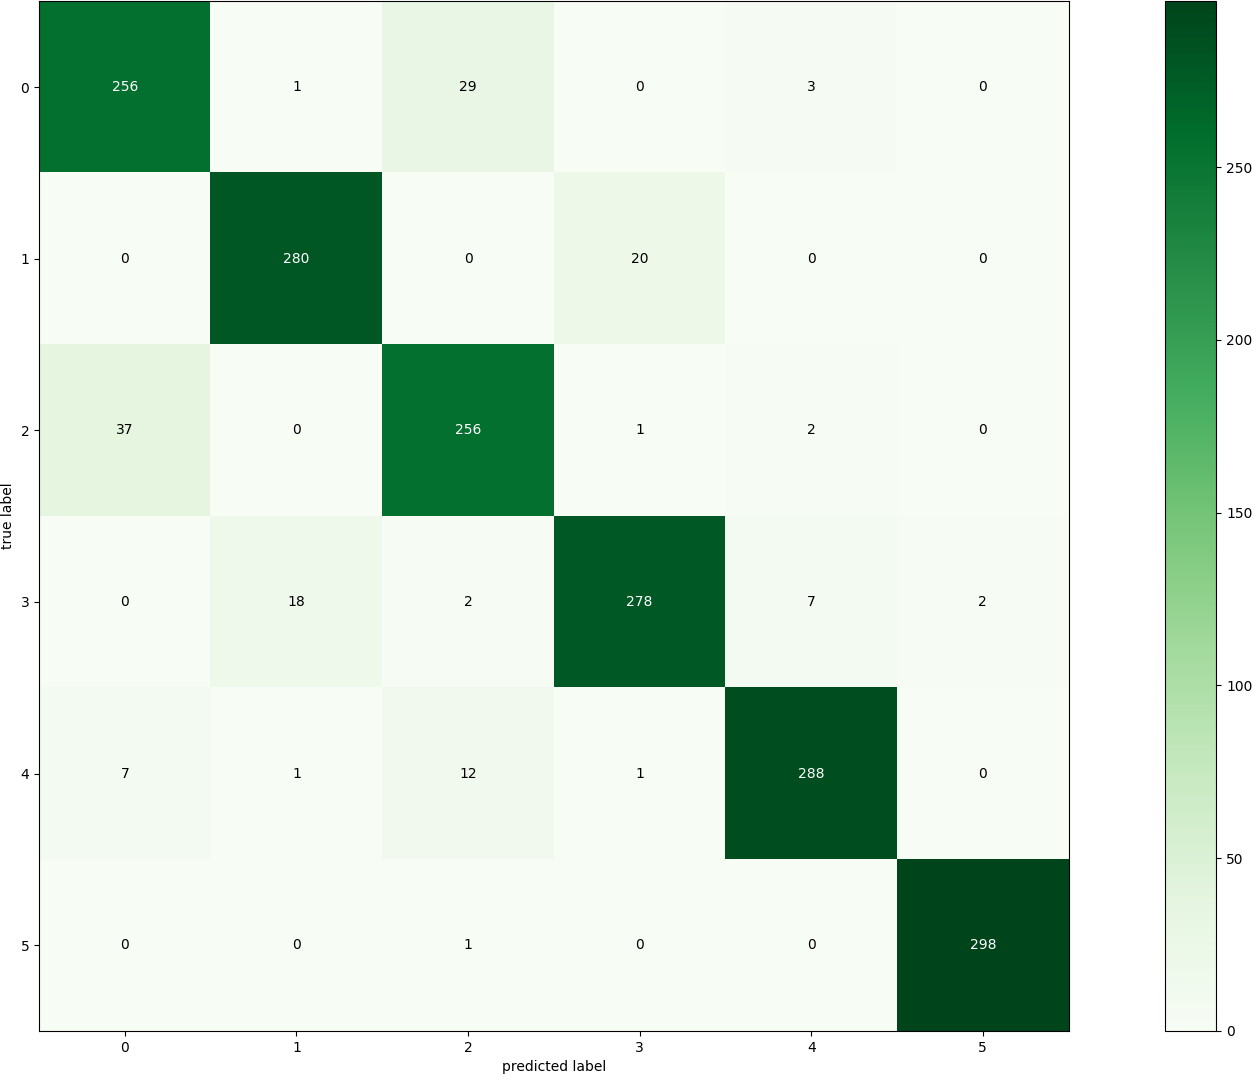
\includegraphics[width=3in]{../images/cm1-test.png}
\captionsetup{justification=centering}                                                                                         
\caption{Confusion matrix on test dataset \\ (cut at \texttt{fc1} + SVM($C=100, \gamma=scale$)))}
\label{fig:cm1-test}                                                                                                                               
\end{figure}

The training phase for SVM took ${\sim550}$ seconds. We tried to simplify the model and thus decrease the timings by reducing the dimensionality of the features. In order to do so we used PCA as technique for dimensionality reduction.


\subsection{Dimensionality Reduction}
In this section we describe how we achieved high accuracy by reducing the dimensionality of the features in input.\par
Before applying PCA, we estimated how many components were needed to describe the data. This can be determined by looking at the \emph{cumulative explained variance} ratio as a function of the number of components.

The curve in Figure \ref{fig:var1} quantifies how much of the total $4096-$dimensional variance is contained within the first $n$ components. For example, we saw that the first ${\sim400}$ components contain approximately $80\%$ of the variance, while are needed around $2\,500$ components to describe $100\%$ of the variance.
\begin{figure}[ht!]
\centering                                                                        
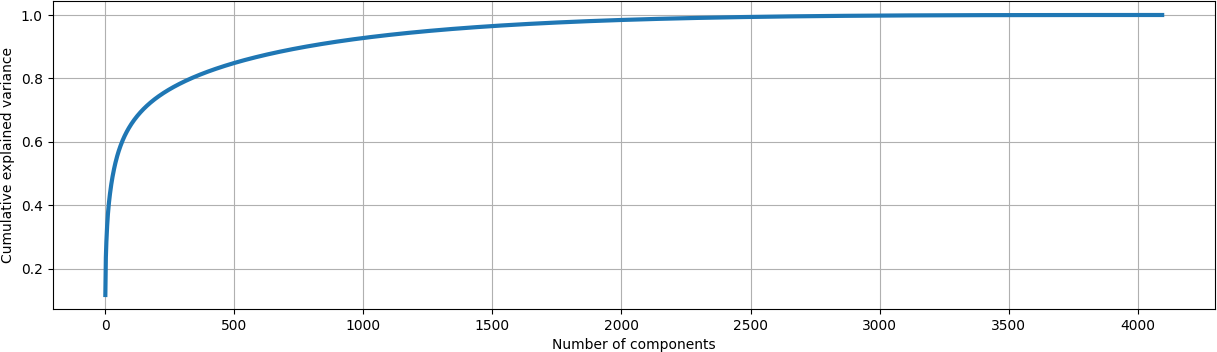
\includegraphics[width=3.5in]{../images/var-1.png}
\captionsetup{justification=centering}                                                                                         
\caption{Confusion matrix on test dataset \\ (cut at \texttt{fc1} + SVM($C=100, \gamma=scale$)))}
\label{fig:var1}                                                                                                                               
\end{figure}
We chose a configuration that could preserve $90\%$ of the variance, \emph{i.e.} $777$ components. This could assure good perfomances while using just $19\%$ of the dimensions.\par
In this case we found the optimal configuration of the SVM with $C=5$ and $\gamma=scale$.

\begin{figure}[ht!]
\centering                                                                        
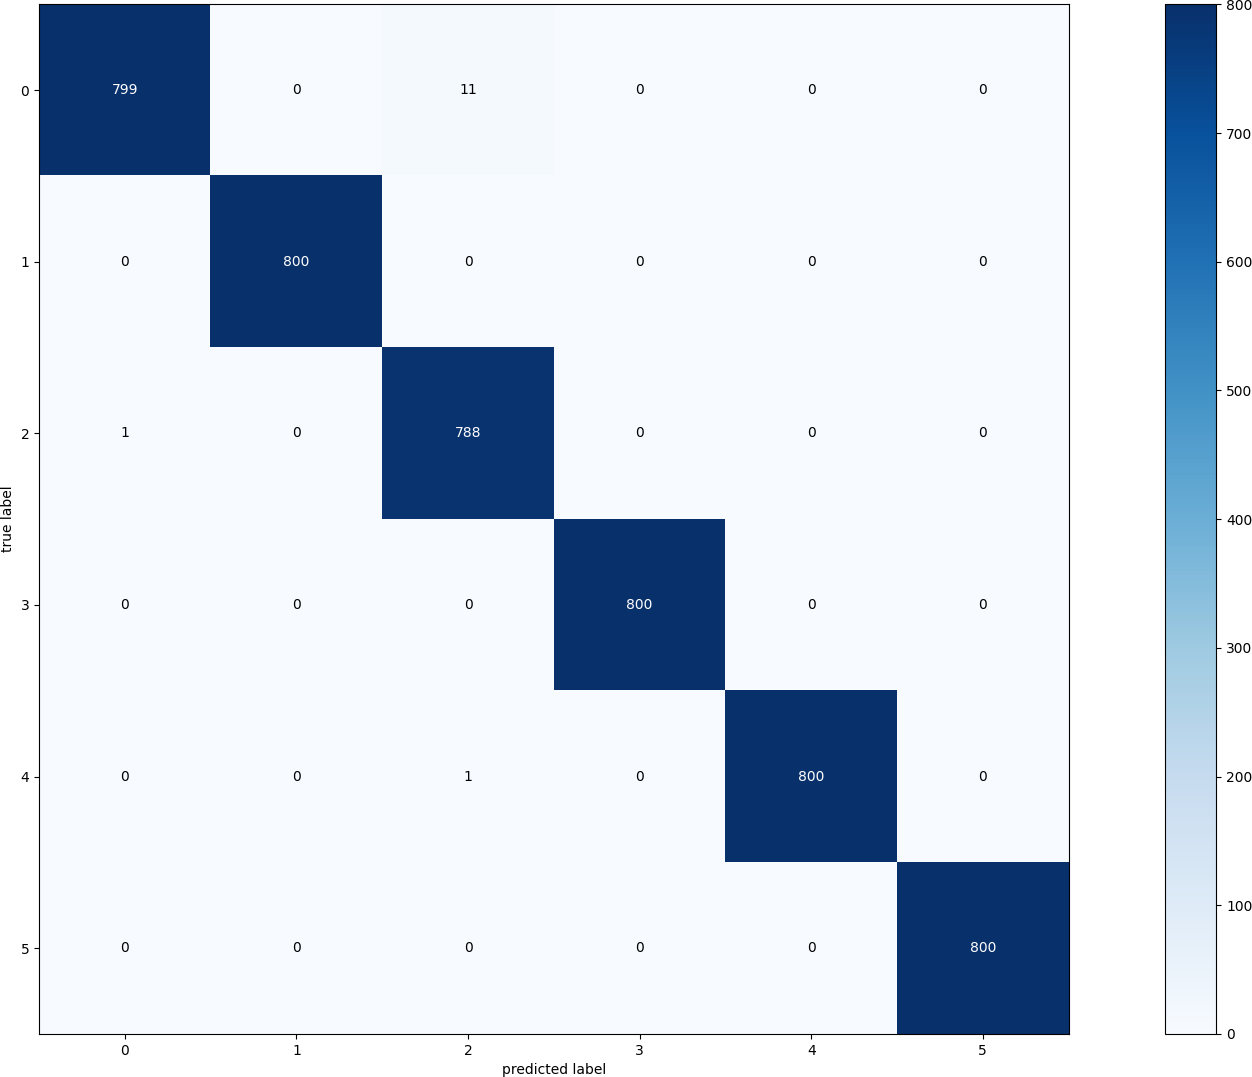
\includegraphics[width=3in]{../images/cm1-pca-train.png}
\captionsetup{justification=centering}                                                                                         
\caption{Confusion matrix on training dataset \\ (cut at \texttt{fc1} + PCA + SVM($C=5, \gamma=scale$))}
\label{fig:cm1-pca-train}                                                                                                                               
\end{figure}


\begin{figure}[ht!]
\centering                                                                        
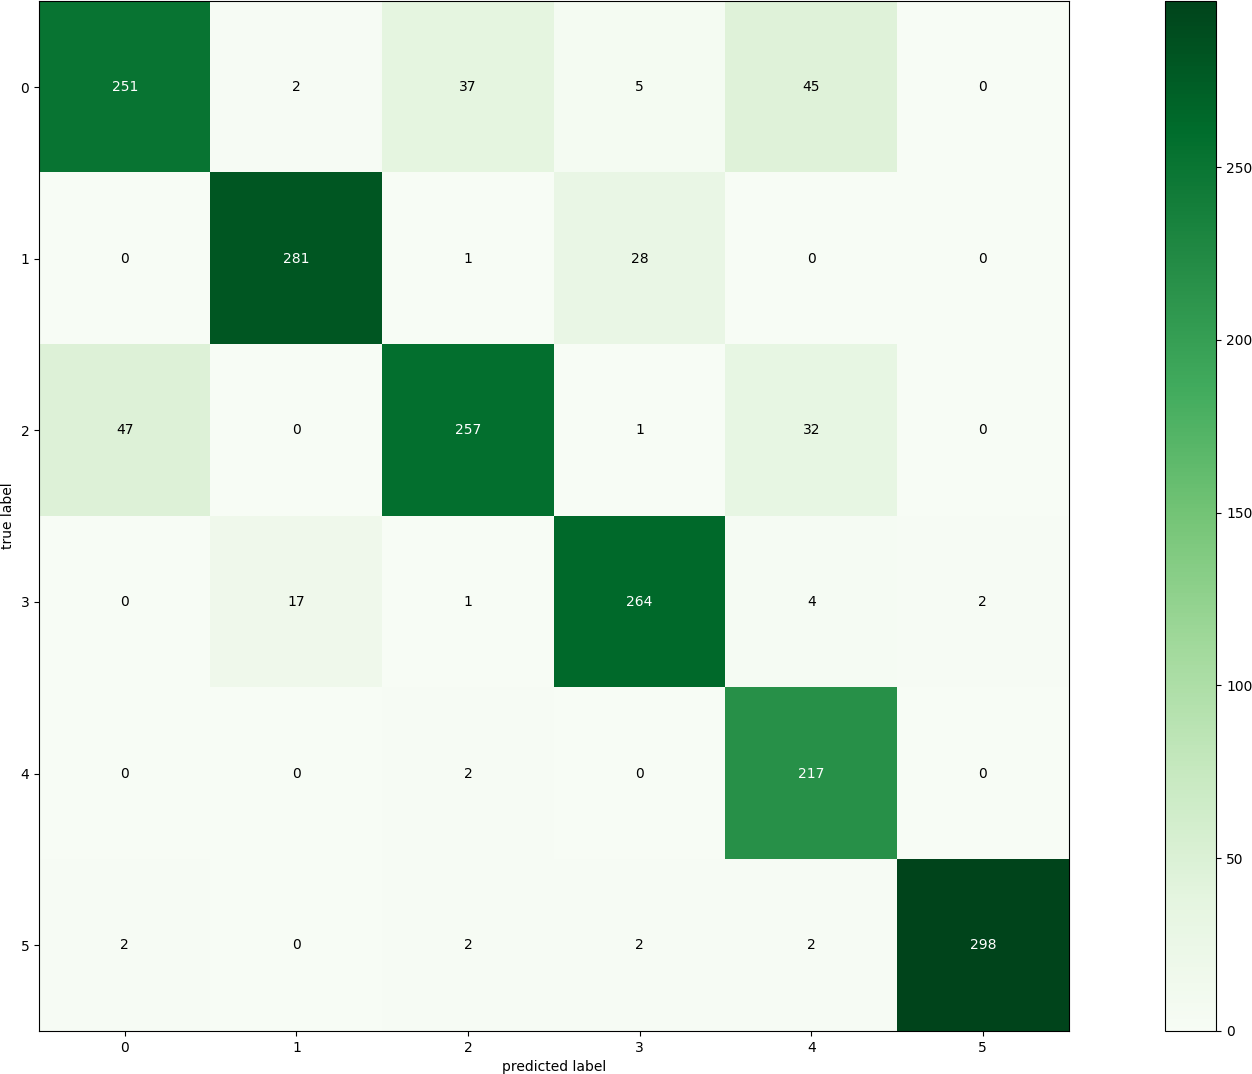
\includegraphics[width=3in]{../images/cm1-pca-test.png}
\captionsetup{justification=centering}                                                                                         
\caption{Confusion matrix on test dataset \\ (cut at \texttt{fc1} + PCA + SVM($C=5, \gamma=scale$))}
\label{fig:cm1-pca-test}                                                                                                                               
\end{figure}
Figure \ref{fig:cm1-pca-train} and \ref{fig:cm1-pca-test} shows the confusion matrix after training and testing. We can see that there is a slight worsening in training accuracy ($99.9\%$) while test accuracy dropped to $88\%$. We noticed that the model still confused glaciers with mountain and streets with buildings; in addition to them, some of the images of the sea are mistaken for mountains and glaciers. That means the model is affected by more overfitting before applying PCA. \par
The lower accuracy and higher overfitting are traded off with faster times in training: we measured a speed up of almost $10$ times, reaching $57$ seconds.












\section{Second cutting point: \texttt{block4\_pool}}

Like in section \ref{sec:fc1} we repeated the experiment of visualizing the features extracted from layer \texttt{block4\_pool} through PCA and plotted the graph in Figure \ref{fig:pca2}.

\begin{figure}[ht!]
\centering                                                                        
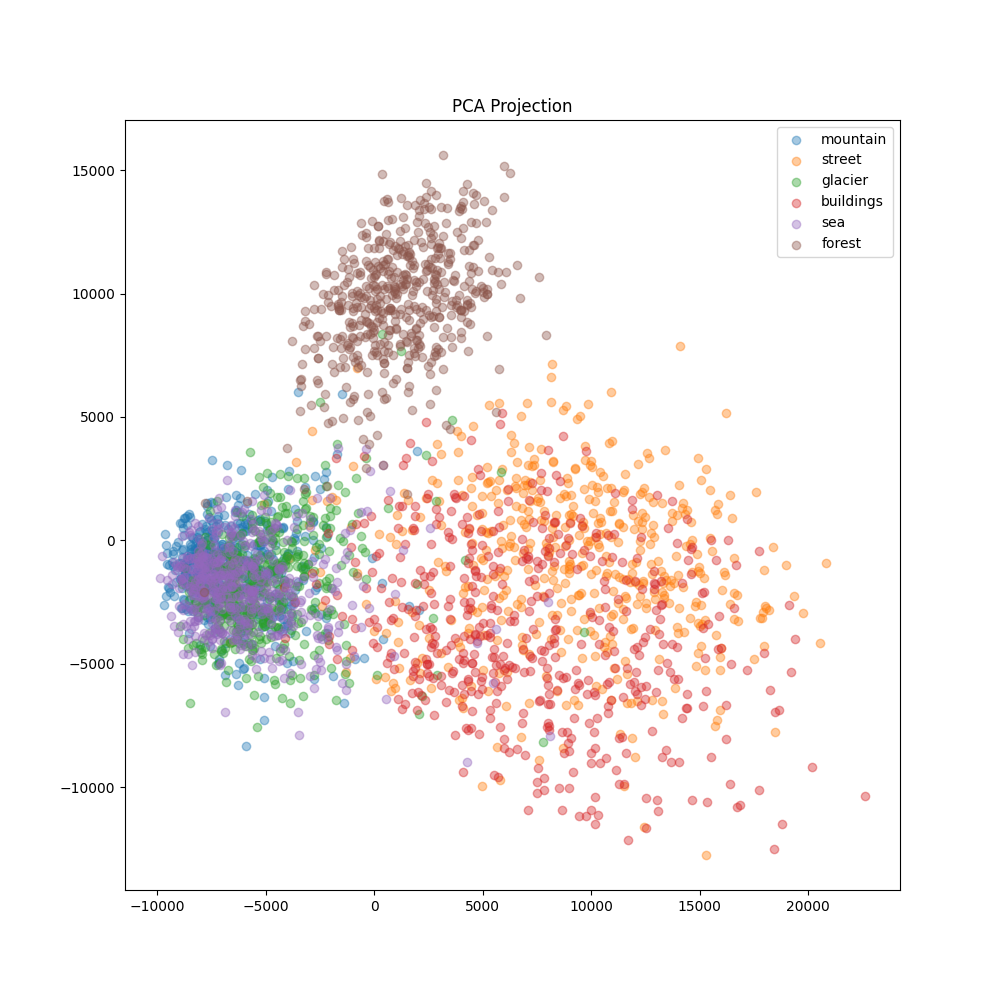
\includegraphics[width=3.5in]{../images/pca-2.png}
\captionsetup{justification=centering}                                                                                         
\caption{Architecture of VGG16 with the cuts applied in this work}
\label{fig:pca2}                                                                                                                               
\end{figure}

This time the sea, glacier and mountain classes collapsed in one cluster. This anticipated that images belonging to these classes could be classified with lower accuracy.
The cluster of images of forest is the only one that did not collide with any other.
We also noticed more isolated images being completely misclassified than the previous cut, \emph{e.g.} some images of mountain or sea are predicted as building or street.




\bibliographystyle{ieeetr}
\bibliography{Bibliography}

\begin{thebibliography}{9}

\bibitem{site1} 
Practice Problem: Intel Scene Classification Challenge \\
\texttt{https://datahack.analyticsvidhya.com/contest/practice-problem-intel-scene-classification-challe}

\bibitem{site2} 
OpenVINO™ documentation \\
\texttt{https://docs.openvino.ai/latest/index.html}

\bibitem{vgg16}
\emph{Very Deep Convolutional Networks for Large-Scale Image Recognition} \\
Karen Simonyan, Andrew Zisserman \\
\texttt{https://doi.org/10.48550/arXiv.1409.1556}

\end{thebibliography}

\end{document}









